\section{Quality plan}

\subsection{Process description and quality management}

\subsubsection{Component development pipeline}
\begin{figure}[H]
    \centering
    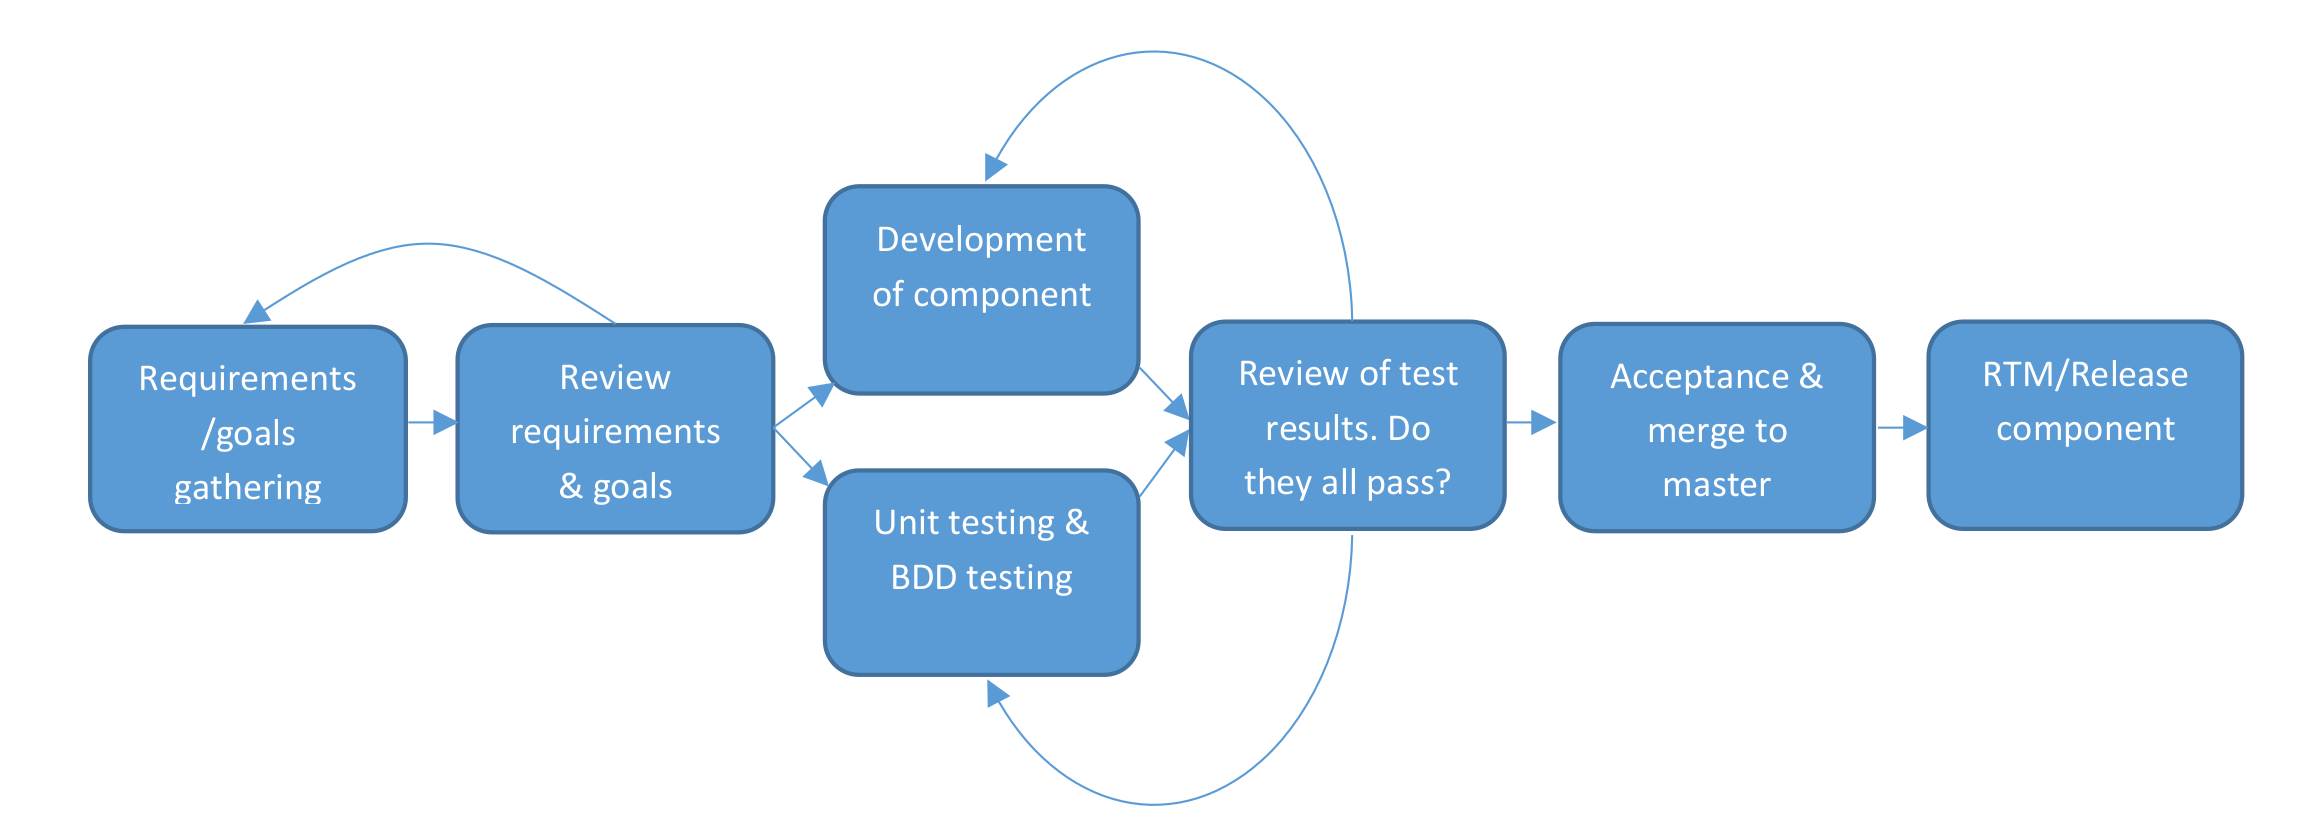
\includegraphics[width=1\textwidth]{images/component_dev_pipeline.png}
    \caption{Component development pipeline}
    \label{componentdevpipeline}
\end{figure}

The first stage of the development pipeline will be to define the goals based on an assessment of the
current situation that has already been done. The goals of the component will be realised by the
requirements and constraints which can be derived from the assessment. Depending on the
individuals involved, requirements can become quite extensive. It is important that, at the start, key
goals are decided on; this will ensure a level of focus when developing the code as these factors
define the definition of done.

As long as goals have been set for the specific component, development can then begin. First
cut/prototypes can be created very quickly and can be built on further after regular reviews of the
progress made. Unit tests, at the very least, should be written along side code that is being
developed. If anything, it may be useful to write the test code before writing the actual methods; a
TDD approach. Either way, it is important to hit a level of code coverage that is agreed on as a
standard. If appropriate for the component being developed, black box testing can also be done
after having a set of tests defined. If time permits, and is defined in the definition of done, BDD
testing can also be included into the testing strategy. Only issue with this is that frameworks may
need to be developed in advance to take advantage of this. BDD testing will be a way have
automated end to end tests in place which can be placed in a CICD pipeline.

Any work that is done and is submitted for review should be judged on the criteria set by the initial
requirements/goals. If submitted work does not meet a specified requirement or goal, then it is to
be rejected with the appropriate comments on why it was rejected. A minimum level of quality, that
needs to be achieved, can also be defined as a requirement to meet the definition of done.

Code reviews can be done on the development branch being used. Release candidates will be taken
from the latest version of master. RTM/Release of the component may be done when a review
meeting is set and stakeholders are satisfied with the level of quality achieved in the latest release
candidate.

\subsection{Testing}
\subsubsection{Performance testing }
To test how stable the server application is, some form of performance testing will be carried out. 
This will also help to find any issues in scalability and optimise the performance. 
Depending on how many clients could be trying to access the server, performance could be seen to be very poor.
Ensuring the software solution is stable under load will ensure that a level of quality and reliability is met.

\subsubsection{Unit testing}
Unit tests will be written along side the main code development. 
A recommended guideline of code coverage between 70 -80\% \cite{cornett2006codecoverage} needs to be set. 
Using software such as SonarQube \cite{sonarqube2017} in a CICD pipeline can raise flags when code coverage drops below the given figure; preventing it 
from being merged to master.

\subsubsection{User acceptance testing}
User acceptance testing (UAT) is the last stage of the software testing process.
A limited number of users will be given access to the system and their usage will determine if the application is able to handle real world 
tasks \cite{techopedia2018uat}.
It can also  be used to evaluate the system's compliance with the initial requirements.
UAT is considered a form of black box testing as the users will have no underlying knowledge of the codebase.

\subsection{Code commenting}
An aim to have a consistent level of commenting. In order to keep the code maintainable, it is
important that other developers can easily figure out what a piece of logic is doing. Another developer should be
able to utilize a previously written program (or function) without ever having to look at the code, simply
by reading the comments \cite{germain2010commenting}.

\subsection{Source control}
To manage the project, proper version control processes should be put in place.
Having a good commit strategy is vital to keeping a record of the work that has been done.
The university hosts their own GitLab instance and will be used as the version control system.
Each day work is done, progress should be detailed in the commit log in a verbose fashion.
It is vital to have detailed commit messages to understand what was done during that development period.
Major features should be worked on branches to avoid ruining the codebase that exists on the master branch.
Merge requests can be used to review work done on a branch and ensure that everything is ok before merging back to master.


\subsection{Continuous integration}
CICD pipelines may be set up using a Jenkins build and/or using the CICD features that are available on
the university Gitlab. The CICD pipelines will be there to carry out all of the unit test and any further
tests that available to run on every commit. This will ensure that the committed code is not breaking
anything. This is a way to continuously regression testing against the code.

%-----------------------------------------------------------------------------------%

\subsection{Quality goals}

\subsubsection{Definitions of quality}
\begin{itemize}
    \tightlist
    \item Quality is fitness for use \cite{asq2005qualityglossary}.
    \item Quality means conformance to requirements \cite{morgan1994total}.
    \item Quality is a degree of excellence...\cite{merriam2007qualitydefinition}
\end{itemize}

\subsubsection{ISO 25010}

\begin{figure}[H]
    \centering
    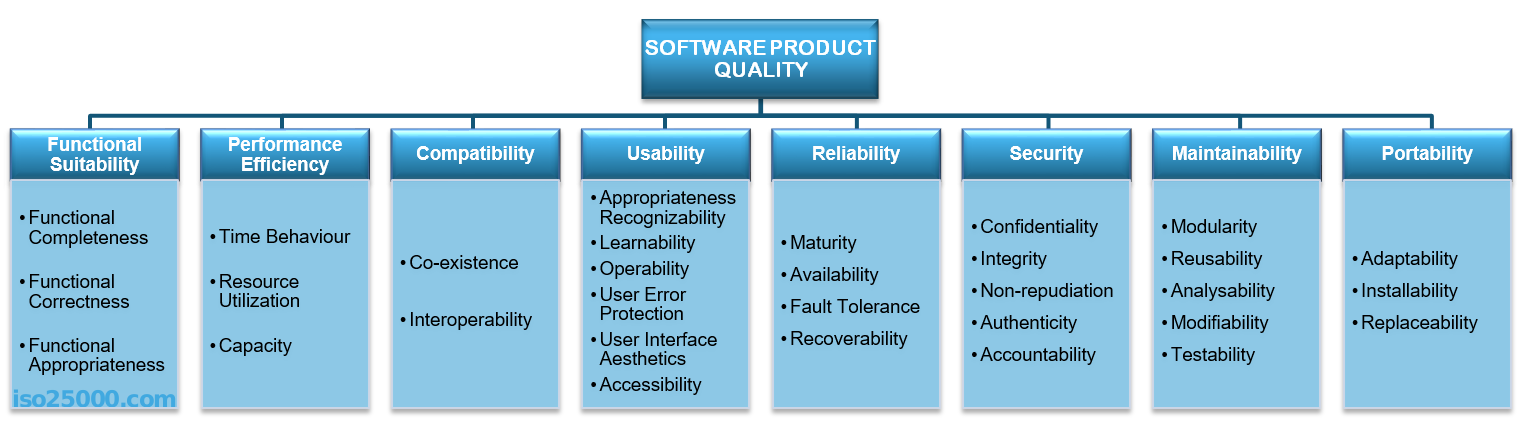
\includegraphics[width=1\textwidth]{images/iso25010.png}
    \caption{Product quality model defined in ISO 25010}
    \label{productquality model}
\end{figure}

The quality of a system is the degree to which the system satisfies the stated and implied needs of
its various stakeholders, and thus provides value. Those stakeholders' needs (functionality,
performance, security, maintainability, etc.) are precisely what is represented in the quality model,
which categorizes the product quality into characteristics and sub-characteristics.

The product quality model defined in ISO/IEC 25010 comprises the eight quality characteristics
shown in the following figure:

\begin{longtable}{|p{.15\textwidth}|p{.85\textwidth}|}
    \hline
    Quality                & Application to the project                                                                                                                                                                                                                                                                                                         \\
    \hline\hline
    Functional suitability & Server and client components perform their jobs as intended. All functionality set out in requirements/specification have been met.                                                                                                                                                                                                \\
    \hline
    Performance efficiency & Components should not use excessive resources to ensure that maximum performance is met with minimal slowdown. Server component should be able to scale well. Client components should make API calls and process responses in a timely manner.                                                                                    \\
    \hline 
    Compatibility          & Client components need to work on a wide range of hardware to attract a large number of users. Should not conflict with any other applications.                                                                                                                                                                                    \\
    \hline
    Usability              & APIs must be well documented and logical. User interfaces must also have the appropriate documentation and be simple to use; over-complicated UI can deter potential users from using the software.                                                                                                                                \\
    \hline
    Reliability            & Components should have reasonably verbose logging that logs the appropriate errors. Server application should be able to recover itself if it crashes.                                                                                                                                                                             \\   
    \hline
    Security               & Only the minum amount of data should be transferred over the network when communicating with the server application. Restrictions/protections should be in place to prevent access to non-user areas.                                                                                                                              \\
    \hline
    Maintainability        & Ensure as much code can be reused between the main web application and the potential Android application. Avoid repeating the same lines of code in multiple places, refer to a common object or configuration file so that values can be changed from a single place.                                                             \\
    \hline
    Portability            & Server and client components need to be compatible with a range of hardware and software combinations as defined in the requirements. E.g. Android application to be compatible with different devices running different versions of android. Individual components should be replacable without modifying or affecting the others.\\
    \hline

    \caption{How ISO 25010 applies to this project}
\end{longtable}


\subsubsection{Maximising code re-use}
To help make the code more more maintainable, it would be really beneficial if code can be reused where appropriate. 
It should be possible to make the web and android applications share code via the use of webviews (or an alternative equivalent). 
This should make the code much more maintainable as will lead to less code being needed to achieve the desired goal. 
It should also ensure that the user experiences are consistent between the web and android applications. 

\subsubsection{Modularity}
Rather than one big blob, this software solution being produced in this project, is broken up into three distinct components.
The entire system, however, still needs to be flexible/adaptable to any changes required in the future such as enhancement requests or 
general bug fixes. 
Consistent coding standards should be maintained while developing the three components. 
Server-side component will be tackled using a microservices architecture. 
This will further allow modularity to the system as it will allow individual services to be self contained. 
It should also enable new services to be added with few issues as long as a standard for structuring the microservices is kept. 

\subsubsection{Security}
Since the web and android applications will be open to the public for use, it is important that measures are put in place to protect user data. 
If any personally identifiable information needs to be collected, then it is important that regulations set out by GDPR are followed to 
protect users \cite{eu2016gdpr}.

\subsubsection{Coding metrics}
During development, to make the lives easier of the developers and code reviewers, it makes sense to adhere to some good practices. 
This will ensure a level of quality is maintained when writing code as well as making it easier to maintain if anything is to be added as an 
enhancement request or fixing defects. 
With software solutions such as SonarQube, checking metrics such as code coverage can be included as part of the CICD pipeline.

\clearpage
\begin{longtable}{|p{.15\textwidth}|p{.70\textwidth}|p{.15\textwidth}|}
    \hline
    Metric                              & Description                                                                                                                                                                                             & Expected value      \\
    \hline\hline
    Method lengths (number of lines)    & Method should be kept as short as possible. If a method becomes too large, it is likely it can be broken down into smaller chunks which are easier to maintain and test.                                & Less than 100 lines \\
    \hline
    Commenting \%                       & Detailed comments should be present to as much of the code as possible. This makes the code easier to understand in the future. Java docs can also be produced which is a valid form of documentation.  & More than 5\%       \\
    \hline
    Code coverage                       & A recommendation is to have code coverage, for the system,between 70\% and 80\%.                                                                                                                        & More than 70\%      \\
    \hline
    Unit test coverage                  & It is recommended to have code coverage, from unit testing, to be around 10\%-20\% higher than system testing.                                                                                          & More than 80\%      \\
    \hline
    Changes per commit                  & Changes per commit should be small, this will ensure that tracing code changes is much simpler. Commits should have the appropriate comments as to what has changed.                                    & Less than 300 lines \\
    \hline
    Inheritance depth                   & Having deep inhertience in code can create confusion to what methods are overridden and may make the logic confusing to follow.                                                                         & Less than 3 levels  \\
    \hline

    \caption{Targeted coding metrics}
\end{longtable}


%---------------------------------------------------------------------------------------%
\subsection{Risks and risk management}
Some of the main potential risks should be raised while gather requirements.
Through, throughout development more potential risks will likely surface so it is important to review them at regular intervals; during
sprint retrospectives for example.

\begin{longtable}{|p{.15\textwidth}|p{.57\textwidth}|p{.10\textwidth}|p{.12\textwidth}|}
    \hline
    Category        & Examples in the context of the project                                              & Impact & Probability   \\
    \hline\hline    
    Functionality   & Features that do not meet the full extent of the requirements.                      & Small  & Small         \\
                    & Features that are never use din the product.                                        & Medium & Small         \\
    \hline  
    Reliability     & One of the components failing in production, prevents users from using the software.& Large  & Small         \\
                    & Operations not exhibiting the expected behaviour, different outputs for same input. & Large  & Small         \\ 
    \hline  
    Useability      & User interface over-complicated for target users.                                   & Large  & Medium        \\
                    & Creating survey feature over-complicated for experts.                               & Large  & Medium        \\
    \hline  
    Efficiency      & System requiring too many resources.                                                & Medium & Small         \\
                    & System taking too long to submit/push/respond to surveys.                           & Medium & Small         \\     
    \hline
    Maintainability & Code too complex, leading to large over head in future development.                 & Large  & Medium        \\
                    & Dependencies used are unreliable.                                                   & Large  & Medium        \\
    \hline
    Performance     & Web/android user interfaces and server side APIs  taking too long to respond.       & Medium & Small         \\
    \hline
    
    \caption{Quality risks categorised according to ISO 9126}
\end{longtable}

